\documentclass[tikz,border=4pt]{standalone}
% Shared TikZ style for lecture figures
\usepackage{amsmath,amssymb}
\usepackage{tikz}
\usetikzlibrary{arrows.meta,calc,decorations.pathreplacing,patterns}
\definecolor{teal}{RGB}{38,150,140}
\definecolor{coral}{RGB}{230,95,75}
\definecolor{ink}{RGB}{20,45,60}
\tikzset{
  >={Stealth[length=2.6mm]},
  every picture/.style={line cap=round,line join=round,thick,ink},
  map/.style={->,thick},
  dot/.style={circle,fill,inner sep=1.2pt},
}

\begin{document}
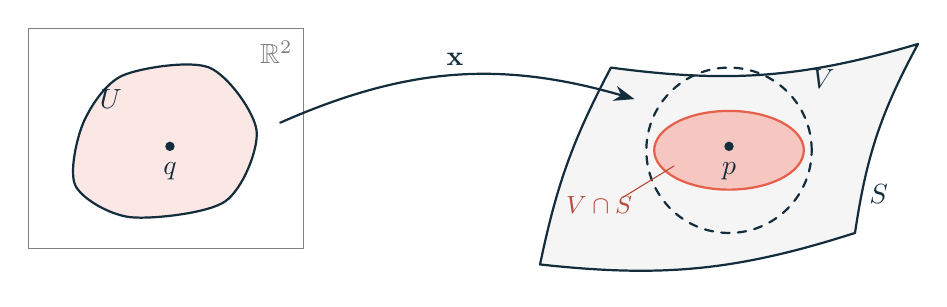
\begin{tikzpicture}
  % parameter domain U in R^2
  \draw[thin,gray] (-0.3,-0.2) rectangle (3.2,2.6);
  \node[gray] at (2.85,2.3) {$\mathbb{R}^{2}$};
  \draw[fill=coral!15] plot[smooth cycle] coordinates {(0.3,0.6) (1.0,0.2) (2.2,0.4) (2.6,1.3) (2.0,2.1) (0.9,2.0) (0.4,1.4)};
  \node at (0.75,1.7) {$U$};
  \node[dot,label=below:{$q$}] (q) at (1.5,1.1) {};
  % surface S in R^3
  \begin{scope}[xshift=6.2cm,yshift=-0.4cm]
    \draw[fill=gray!8] (0,0) to[bend right=12] (4,0.4) to[bend left=10] (4.8,2.8)
      to[bend left=12] (0.9,2.5) to[bend right=8] cycle;
    \node at (4.3,0.9) {$S$};
    \draw[dashed] (2.4,1.45) circle (1.05);
    \node at (3.6,2.35) {$V$};
    \draw[fill=coral!35,draw=coral] (2.4,1.45) ellipse (0.95 and 0.5);
    \node[dot,label=below:{$p$}] (p) at (2.4,1.5) {};
    \node[coral!80!black] at (0.75,0.75) {\small $V\cap S$};
    \draw[coral!80!black,thin] (1.05,0.85) -- (1.7,1.25);
  \end{scope}
  \draw[map] (2.9,1.4) to[bend left=20] node[above] {$\mathbf{x}$} (7.4,1.7);
\end{tikzpicture}
\end{document}
